\documentclass[10pt,conference]{IEEEtran}

\usepackage[hidelinks]{hyperref}
\usepackage{microtype}
\usepackage{graphicx}
\usepackage{amsmath}
\usepackage{booktabs}
\usepackage{pgfplots}
\pgfplotsset{compat=1.16}

% 5-fold cross-validation, F1 in % (mean $\pm$ std over folds),
% from report/results.json, key "cv".
\newcommand{\cvMin}{$41.6\pm0.7$}
\newcommand{\cvRidge}{$41.9\pm0.8$}
\newcommand{\cvFull}{$43.0\pm0.8$}
\newcommand{\cvSel}{$42.8\pm1.0$}

\begin{document}
\title{Coronary Heart Disease Prediction from Survey Data}

\author{
\IEEEauthorblockN{[Team member 1], [Team member 2], [Team member 3]}
\IEEEauthorblockA{CS-433 Machine Learning, EPFL, Switzerland}


}

\maketitle

\begin{abstract}
This paper investigates the prediction of self-reported coronary heart
disease using 321 variables from the 2015 BRFSS health survey and linear
models implemented in NumPy. With a positive-class prevalence of 8.8\%,
we adopt F1 as the primary evaluation metric. Survey-specific cleaning
and encoding yield 836 features. Regularised logistic regression with a
training-selected decision threshold achieves \cvFull{} F1 in five-fold
cross-validation, versus \cvMin{} with minimal preprocessing. Ablation
experiments indicate that decision-threshold selection contributes
substantially more than any individual preprocessing operation.

\end{abstract}

\section{Introduction}
The Behavioral Risk Factor Surveillance System (BRFSS) collects US
telephone-survey responses concerning health behaviours and chronic
conditions~\cite{brfss}. The prediction target is self-reported coronary
heart disease or myocardial infarction (MICHD), using 321 survey
variables. The dataset comprises 328{,}135 labelled training respondents
and 109{,}379 test respondents. Positive cases account for only 8.8\% of
the labelled sample. Therefore, a majority-class classifier attains
approximately 91\% accuracy while detecting no positive cases. We
accordingly report positive-class F1, the competition evaluation metric,
in percent. This study compares six independently implemented linear methods,
develops a preprocessing strategy informed by BRFSS response coding, and
quantifies the contributions of its components through ablation.
Because the outcome is self-reported, these predictions characterise
survey responses rather than confirmed diagnoses or
prospective clinical events.

\section{Methodology}

\subsection{Linear prediction methods}
All six estimators were implemented in \texttt{implementations.py} and
passed the public tests. Ordinary linear regression minimises
$\frac{1}{2N}\|y-Xw\|^2$ using full-batch gradient descent (GD),
single-sample stochastic gradient descent (SGD), or the closed-form
normal equations. Ridge regression introduces a $\lambda\|w\|^2$
penalty and solves $(X^\top X+2N\lambda I)w=X^\top y$. Logistic
regression is optimised by GD, both with and without this penalty.
Targets are represented as $\{0,1\}$; continuous model outputs are
subsequently thresholded to obtain binary predictions.

\subsection{Survey data characteristics}
Conditional question routing produces substantial missingness: 99 of 321
variables are unobserved for at least 90\% of respondents. Such patterns
may carry predictive information. Six variables are constant whenever
observed. Additionally, 273 variables contain
codes including 7, 9, 77, and 99. These frequently indicate
``don't know'' or ``refused'', although meanings depend on the field:
for example, income code 7 represents the \$50--75k category.
Thus, applying uniform non-response rules could discard valid
observations and introduce systematic errors into feature construction.

\subsection{Feature preprocessing}
Preprocessing parameters are estimated exclusively from training data.
\begin{enumerate}
\item \emph{Variable exclusion.} We discard 43 fields by hand: 18 describing interview administration
rather than respondents (e.g.\ dates or survey weights), 11 redundant
or almost empty variables, and 14 raw unit-encoded answers with
existing decoded equivalents (e.g.\ 107 encodes seven days per week in
\texttt{ALCDAY5}). We additionally drop 27 fields with at least 99\%
missing observations.
\item \emph{Non-response handling.} Field-specific missing-value codes
are identified using training observations: 77/99 when available,
otherwise 777/999, otherwise 7/9, except where the codebook identifies
7 as a legitimate category. These responses are treated as missing;
code 88 (``none'') is recoded to zero for count variables.
\item \emph{Feature representation.} The 180 categorical fields
(nominal, or containing at most ten levels) use $k-1$ dummy variables
and include missingness as an explicit category. Seven ordinal and
60 continuous fields are median-imputed, standardised, and accompanied
by missingness indicators. Six constant-valued fields are represented
solely through their observation indicators.
\end{enumerate}


\subsection{Experimental protocol}
For the positive class, precision is $P=TP/(TP+FP)$, recall is
$R=TP/(TP+FN)$, and F1 is $F_1=2PR/(P+R)$. The decision threshold
satisfies $t\in[0,1]$.
The primary classifier is regularised logistic regression, initialised
at $w=0$ and trained using GD. A prediction is positive when its
estimated probability exceeds threshold $t$, selected to maximise F1.
Hyperparameters were evaluated on a random 80/20 split (seed 2026):
$\lambda\in\{10^{-5},10^{-4},10^{-3}\}$,
$\gamma\in\{0.03,0.1,0.3,0.6\}$, and
$T\in\{500,1000,3000\}$ iterations. To prevent validation-label
optimism, thresholds are fitted using training predictions only. The
principal comparison is additionally evaluated by five-fold
cross-validation, with preprocessing refitted within each training fold.
Ablation uncertainty is estimated from 1000 paired bootstrap resamples
using 95\% intervals. All experiments are reproducible through
\texttt{report/experiments.py}.

\section{Results and Analysis}

\begin{table}[tbp]
\centering
\caption{Hold-out comparison of linear methods and five-fold CV
F1 (mean $\pm$ standard deviation), all in \%. All models use 836
features except the minimal baseline. Logistic models use $\gamma=0.3$
and $T=1000$ (selected variant: $\gamma=0.6$, $T=3000$); regularised
models use $\lambda=10^{-4}$}
\label{tab:methods}
\footnotesize
\setlength{\tabcolsep}{3.5pt}
\begin{tabular}{@{}lccccc@{}}
\toprule
Method & F1 & Prec. & Rec. & Acc. & CV F1\\
\midrule
Majority class                & 0.0  & --   & 0.0  & 90.9 & --\\
Least squares (normal eq.)    & \multicolumn{5}{c}{non-unique; $X^\top X$ singular}\\
Least squares (GD)            & 42.7 & 34.5 & 56.0 & 86.4 & --\\
Least squares (SGD)           & 42.7 & 35.3 & 53.9 & 86.9 & --\\
Ridge regression              & 42.5 & 35.5 & 53.0 & 87.0 & \cvRidge\\
Logistic regression           & 44.1 & 37.5 & 53.4 & 87.7 & --\\
Reg.\ logistic regression     & 44.1 & 36.3 & 56.1 & 87.1 & \cvFull\\
Reg.\ logistic (selected)     & 44.2 & 36.3 & 56.3 & 87.1 & \cvSel\\
\midrule
Reg.\ logistic (minimal)      & 42.3 & 35.6 & 52.0 & 87.1 & \cvMin\\
\bottomrule
\end{tabular}
\end{table}

\begin{table}[tbp]
\centering
\caption{Single-component ablations on the hold-out split
(regularised logistic regression; $\lambda=10^{-4}$, $\gamma=0.3$,
$T=1000$). Differences in F1 are measured against the full pipeline;
brackets give 95\% paired bootstrap intervals}
\label{tab:ablation}
\footnotesize
\setlength{\tabcolsep}{4pt}
\begin{tabular}{@{}lrcc@{}}
\toprule
Variant & Feat. & F1 & $\Delta$F1 [95\% interval]\\
\midrule
Full pipeline                    & 836  & 44.11 & --\\
No dummy encoding                & 486  & 43.63 & $-0.48$ [$-0.88$, $-0.09$]\\
No missingness indicators        & 772  & 43.91 & $-0.19$ [$-0.48$, $+0.09$]\\
No non-response decoding         & 1060 & 43.99 & $-0.11$ [$-0.46$, $+0.19$]\\
Keep $\ge$99\%-missing columns   & 959  & 43.97 & $-0.14$ [$-0.46$, $+0.20$]\\
Keep interview metadata          & 865  & 44.00 & $-0.10$ [$-0.30$, $+0.10$]\\
Earlier pipeline version         & 844  & 44.09 & $-0.01$ [$-0.19$, $+0.16$]\\
Minimal preprocessing            & 315  & 42.28 & $-1.82$ [$-2.41$, $-1.27$]\\
Fixed threshold $t=0.5$          & 836  & 23.93 & $-20.2$ [$-21.5$, $-18.8$]\\
\bottomrule
\end{tabular}
\end{table}

Table~\ref{tab:methods} summarises the estimator comparison under consistent experimental conditions. The
unregularised normal-equation solution is non-unique because
$X^\top X$ is singular: several columns are linearly dependent. Ridge
regression, GD with step size $1/L$ ($L=76.3$, the largest eigenvalue
of $X^\top X/N$), and SGD with step size $10^{-4}$ for one data pass
obtain F1 scores of 42.5--42.7. Logistic loss improves performance by
approximately 1.5 points. Regularisation provides little additional
benefit: $\lambda=0$ yields F1 44.1, while ridge performance changes
by only 0.1 points for $\lambda\in[10^{-6},10^{-2}]$.
With 262{,}508 training examples and 837 parameters, training F1 (43.1)
is below validation F1, providing limited evidence of overfitting.
The remaining error may instead reflect restricted linear expressiveness.
These results suggest that the objective function matters more than
the optimisation procedure.

For $\gamma\le 0.3$, increasing $\gamma T$ raises validation F1 until
performance stabilises at 43.9--44.3 for $\gamma T\ge 300$;
varying $\lambda$ changes F1 by at most 0.2 points. By contrast, five
of nine runs at $\gamma=0.6$ achieve only F1 26--35. Since logistic-loss
curvature is bounded by $L/4$, a standard GD convergence guarantee
requires $\gamma<8/L\approx 0.1$. Even the best initially selected
$\gamma=0.6$ configuration has higher training loss than $\gamma=0.3$
(0.233 versus 0.219) and lower CV F1 by 0.2 points. Therefore, the
reported primary configuration uses $\gamma=0.3$ and $T=1000$.

\begin{figure}[tbp]
\centering
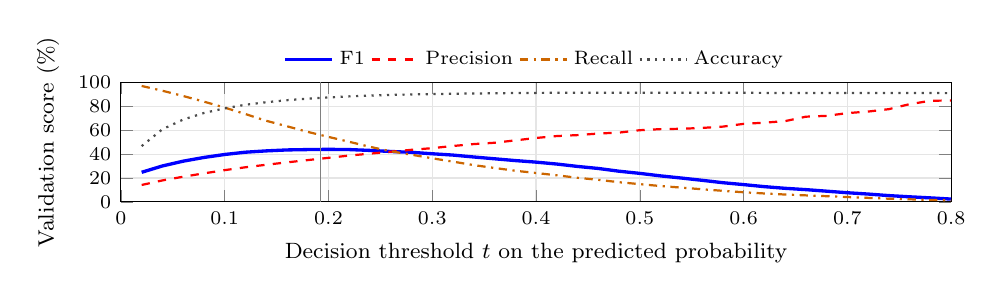
\begin{tikzpicture}
\begin{axis}[
 width=\columnwidth, height=3.1cm,
 xmin=0, xmax=0.8, ymin=0, ymax=100,
 xlabel={Decision threshold $t$ on the predicted probability},
 ylabel={Validation score (\%)},
 tick label style={font=\scriptsize},
 label style={font=\footnotesize},
 legend style={font=\scriptsize, draw=none, at={(0.5,1.02)},
               anchor=south, legend columns=4},
 grid=major, grid style={gray!20},
]
\addplot[very thick, blue] coordinates {(0.02,24.8) (0.04,30.1) (0.06,34.1) (0.08,37.2) (0.1,39.7) (0.12,41.6) (0.14,42.7) (0.16,43.5) (0.18,43.8) (0.2,44.0) (0.22,43.8) (0.24,43.1) (0.26,42.2) (0.28,41.5) (0.3,40.3) (0.32,39.2) (0.34,37.6) (0.36,36.1) (0.38,34.6) (0.4,33.3) (0.42,31.7) (0.44,29.7) (0.46,28.0) (0.48,25.7) (0.5,23.9) (0.52,21.8) (0.54,20.0) (0.56,18.1) (0.58,16.1) (0.6,14.5) (0.62,12.8) (0.64,11.4) (0.66,10.3) (0.68,9.0) (0.7,7.7) (0.72,6.6) (0.74,5.3) (0.76,4.3) (0.78,3.4) (0.8,2.4)};
\addlegendentry{F1}
\addplot[thick, red, dashed] coordinates {(0.02,14.2) (0.04,18.0) (0.06,21.1) (0.08,23.9) (0.1,26.6) (0.12,29.0) (0.14,31.1) (0.16,33.1) (0.18,35.0) (0.2,36.9) (0.22,38.8) (0.24,40.4) (0.26,42.0) (0.28,43.6) (0.3,45.0) (0.32,46.8) (0.34,48.4) (0.36,49.5) (0.38,51.5) (0.4,53.5) (0.42,55.1) (0.44,55.9) (0.46,57.2) (0.48,58.0) (0.5,60.0) (0.52,60.9) (0.54,61.2) (0.56,61.9) (0.58,63.0) (0.6,65.3) (0.62,66.3) (0.64,67.6) (0.66,71.3) (0.68,72.0) (0.7,74.3) (0.72,75.6) (0.74,77.6) (0.76,81.8) (0.78,84.6) (0.8,84.9)};
\addlegendentry{Precision}
\addplot[thick, orange!80!black, dash dot] coordinates {(0.02,97.0) (0.04,93.0) (0.06,88.6) (0.08,83.9) (0.1,78.9) (0.12,73.5) (0.14,67.9) (0.16,63.3) (0.18,58.6) (0.2,54.4) (0.22,50.3) (0.24,46.1) (0.26,42.4) (0.28,39.5) (0.3,36.5) (0.32,33.7) (0.34,30.8) (0.36,28.4) (0.38,26.1) (0.4,24.2) (0.42,22.3) (0.44,20.2) (0.46,18.5) (0.48,16.5) (0.5,14.9) (0.52,13.3) (0.54,12.0) (0.56,10.6) (0.58,9.3) (0.6,8.1) (0.62,7.1) (0.64,6.2) (0.66,5.5) (0.68,4.8) (0.7,4.1) (0.72,3.4) (0.74,2.7) (0.76,2.2) (0.78,1.7) (0.8,1.2)};
\addlegendentry{Recall}
\addplot[thick, black!70, dotted] coordinates {(0.02,46.7) (0.04,60.8) (0.06,68.9) (0.08,74.4) (0.1,78.3) (0.12,81.3) (0.14,83.4) (0.16,85.1) (0.18,86.4) (0.2,87.4) (0.22,88.3) (0.24,88.9) (0.26,89.5) (0.28,89.9) (0.3,90.2) (0.32,90.5) (0.34,90.7) (0.36,90.9) (0.38,91.1) (0.4,91.2) (0.42,91.3) (0.44,91.3) (0.46,91.3) (0.48,91.3) (0.5,91.4) (0.52,91.4) (0.54,91.3) (0.56,91.3) (0.58,91.3) (0.6,91.3) (0.62,91.2) (0.64,91.2) (0.66,91.2) (0.68,91.2) (0.7,91.2) (0.72,91.1) (0.74,91.1) (0.76,91.1) (0.78,91.1) (0.8,91.0)};
\addlegendentry{Accuracy}
\draw[gray, thin] (axis cs:0.192,0) -- (axis cs:0.192,100);
\end{axis}
\end{tikzpicture}
\caption{Precision, recall, F1, and accuracy for regularised
logistic regression across classification thresholds. The vertical
marker indicates the training-selected operating point ($t=0.192$)}
\label{fig:threshold}
\end{figure}

Figure~\ref{fig:threshold} illustrates the effect of operating point across evaluation metrics.
At $t=0.5$, only 2.3\% of respondents receive a positive prediction;
recall is approximately 15\% and F1 is 23.9, notwithstanding accuracy
near its maximum of 91.4\%. Around $t=0.2$, F1 reaches its optimum,
with approximately 36\% precision and 56\% recall. The threshold
estimated from training predictions closely matches this operating
point. Optimising directly on validation labels would inflate F1 by
only 0.04 points.



Table~\ref{tab:ablation} isolates each preprocessing decision in controlled comparisons. Relative
to the full representation, minimal preprocessing reduces F1 by
1.82 points. Among individual component removals, only disabling dummy
encoding has a 95\% interval excluding zero ($-0.48$ points). Without
this transformation, nominal variables such as employment status are
incorrectly interpreted as ordered numerical quantities. Effects from
other procedures overlap: one-hot columns already distinguish missing
responses and non-response categories, leaving explicit decoding and
missingness indicators most relevant to the 67 ordinal and continuous
variables. An earlier pipeline using shared non-response codes across
variables yields nearly identical performance. Across all five CV folds,
the full pipeline exceeds the minimal baseline by 0.9--1.8 points.
Because the selected hold-out split is relatively favourable, aggregate
CV performance provides a more representative comparison. 

\section{Discussion and Conclusion}
The largest-magnitude coefficients correspond to sex, age, prior stroke,
self-rated general health, chronic pulmonary and kidney conditions, and
blood-pressure medication. Accordingly, the model assigns elevated risk
to respondents with associated health profiles, although coefficients
do not establish causal relationships. Similar F1 scores across the
linear estimators suggest that additional improvements may depend on
nonlinear structure or interaction features rather than hyperparameter
adjustments alone. Overall, survey-aware preprocessing improves
cross-validated F1 by roughly 1.5 points, while decision-threshold
selection yields an improvement of approximately 20 points.
Independent external validation remains necessary before deployment in
any clinical decision-making context.

\begin{thebibliography}{1}
\bibitem{brfss}
Centers for Disease Control and Prevention, ``Behavioral Risk Factor
Surveillance System, 2015 survey data and codebook,''
\url{https://www.cdc.gov/brfss/annual_data/annual_2015.html}.
\end{thebibliography}

\end{document}

